% 言語処理学会年次大会 予稿(v0.2 の LaTeX 整形版)
% -------------------------------------------------------------
% 注意: 年次大会の公式スタイルファイル(例: nlp2027.sty)は CFP 公開時に
% https://www.anlp.jp/ から配布される。入手後は下の「公式スタイル差し替え点」
% に従い \usepackage{nlp2027} へ切り替えるだけで本文はそのまま使える。
% 本ファイルは公式配布までの互換整形(uplatex + jarticle 二段組・A4・
% 本文 4 ページ)である。コンパイル: uplatex → dvipdfmx
% -------------------------------------------------------------
\documentclass[a4paper,twocolumn,10pt]{jarticle}
\usepackage[dvipdfmx]{graphicx}
\usepackage{booktabs}
\usepackage{geometry}
\geometry{top=30mm,bottom=25mm,left=20mm,right=20mm} % ← 公式スタイル差し替え点(公式値に従う)
\setlength{\columnsep}{7mm}
\usepackage{titlesec}
\titleformat*{\section}{\large\bfseries}
\titleformat*{\subsection}{\normalsize\bfseries}
\pagestyle{empty}

\title{\textbf{構成によるラベルは観測から識別不能でありうる:\\手書き風合成答案による数学誤り診断 VLM の学習}}
\author{和山 亮介 \quad Fable 5\\
株式会社ノーザンシステムサービス\\
\texttt{\{r-wayama\}@nssv.co.jp}} % ← メールアドレスは投稿前に確認・修正
\date{}

\begin{document}
\maketitle
\thispagestyle{empty}

\section*{概要}
手書き数学答案の誤り診断を行う視覚言語モデル(VLM)の訓練には,誤りの位置・種別・点数が付与された答案画像が必要だが,そのような細粒度ラベル付き実データは入手困難である.本研究は,解法を実行可能プログラムとして生成し,誤りをプログラム変異として注入し,決定論的レンダリングで答案画像を合成する label-by-construction パイプラインを構築した.9,204 件の合成データによる SFT で,ゼロショットでは全く創発しない誤り位置特定(IoU@0.5 0.000$\rightarrow$0.795)を確立し,幻覚率を 31.4\% から 0\% に抑えた.一方で,構成的には正しいラベルが\textbf{観測からは識別不能}でありうるという合成データ固有の失敗モードを,生成器の全件走査により定量化した:概念的誤解ラベルの 95.6\% が機械的誤記ラベルと答案表面で文字列一致し,種別一致率の未達(0.760)は識別不能部分の多数側タイブレークを仮定した条件付き期待値(0.759)とほぼ一致した.正解を「観測から識別可能な最も細かいラベル」へ写像し,識別不能事例への細粒度断定を過剰主張として罰する評価規約を導入すると,\textbf{再訓練なしの推論時ラベル写像だけで}種別一致 0.970・過剰主張 0\% が得られ,未見問題群でも過剰主張率 90\%$\rightarrow$1\% の低減を確認した.

\section{はじめに}
記述式数学答案の自動採点には,最終解の正誤だけでなく,途中式のどこで・どの種類の誤りが生じたかの診断が求められる.実答案の画像自体は大量に存在するが,誤り位置の座標・細粒度の誤り種別・誤りの伝播・対照(誤りなし)画像を併せ持つ訓練データは,我々が利用可能な範囲には存在しない.人手注釈で賄う場合,1 ページあたり 10 分・時給 2,000 円を仮定すると 1 万ページで約 330 万円に達する.本研究はこの供給問題を\textbf{構成による正解(label by construction)}で解決する:解法を実行可能なステップ列として生成し,誤りを検証可能なプログラム変異として注入し,レンダリングにより全文字の座標を既知とする(図~\ref{fig:pipeline}).

本稿の貢献は 3 点である.
\begin{enumerate}
\item \textbf{パイプライン}:解法プログラム変異・二段ゲート(実行検証/差分封じ込め)・合成方式逐語化(LLM は式に接続する説明句のみを生成し,式はテンプレートから機械合成)・訓練前の報酬敵対的テストからなる実装.9,204 件の SFT により,ゼロショット 0 の誤り位置特定・種別分類を確立した(\S\ref{sec:exp1}).
\item \textbf{失敗モードの定量化と帰属}:構成的に正しいラベルが観測から識別不能でありうることを,生成器出力の全件走査で定量化した(観測同値率 $\rho=0.956$).合成データでは曖昧性の量が生成器の実装から厳密に計算可能であり,「生成経路(provenance)を予測ターゲットにした」という設計上の誤りとして帰属・修正できることを示した(\S\ref{sec:exp2}).
\item \textbf{処方}:正解を観測から識別可能な最も細かいラベルへ写像し,識別不能事例への細粒度断定を\textbf{過剰主張}として罰する評価・報酬規約.再訓練を要しない推論時のラベル写像だけで種別一致 0.970・過剰主張 0\% を達成した.「判別できないときに判別できないと言う」挙動は,根拠なく概念的誤解と断定しない教育的に望ましい採点者の性質に対応する.
\end{enumerate}

\section{関連研究}
\textbf{合成文書データ}:合成レンダリングによる訓練データ生成は SynthText~\cite{gupta2016}, SynthDoG(Donut)~\cite{kim2022} などで広く用いられるが,これらは転記の教師信号を合成する.本研究は誤り位置・種別・採点という反実仮想的な細粒度ラベルを構成により生成する.
\textbf{数学誤り診断}:同一の誤答表面が複数の手続きバグから生じ答案のみからは同定できないこと(診断的曖昧性)は BUGGY~\cite{brown1978}以来知られる.誤りステップ特定~\cite{zheng2025,daheim2024},手書き数学の VLM 評価(FERMAT~\cite{nath2025},CHECK-MAT~\cite{khrulev2025})は活発だが,訓練用の座標付き細粒度ラベルの供給は扱われていない.日本語手書きを含むシーンテキスト理解には JaWildText~\cite{maeda2026} がある.
\textbf{粗い粒度への後退と部分ラベル}:階層上で過剰に細かい予測を罰する枠組み~\cite{deng2012},観測同値な候補集合をラベルとする部分ラベル学習~\cite{cour2011},確信度軸の選択的予測~\cite{chow1970,geifman2017}が知られる.\textbf{本研究の新規性はこれらの概念の提案ではなく},生成器側の曖昧性を全件走査で厳密に定量化し,決定論的述語による再ラベルで修正した点にある.
\textbf{合成データの品質}:factuality・忠実性の課題は整理されている~\cite{liu2024}が,「構成的に正しいが観測から識別不能」という失敗モードの実測・修正の報告は我々の知る限り存在しない.

\section{合成パイプライン}\label{sec:pipeline}
図~\ref{fig:pipeline} に全体を示す.\textbf{M1}:中学 1 年数学 2 領域(正負の数・一次方程式)の問題と模範解答を実行可能なステップ列として生成し,実行により全中間値を検証する(G1a).\textbf{M2}:誤りをステップ列へのプログラム変異として注入する(機械的オペレータと,LLM が誤解に基づく誤り式を提案し AST ホワイトリスト検証を経る概念オペレータ).変異後の再実行と差分封じ込めを G2 が保証し,対照群(誤りなし)を 30\% 混入する.双子ペアは変異サイトより前のステップの字面を完全に共有する(全 3,000 ペアで一致率 100\%).\textbf{逐語化(合成方式)}:LLM の出力は説明句に限定し,式はテンプレートから機械合成する(G1b).式の忠実性が構成的に保証される(プロンプト指示方式は通過率 8/20〜16/20 と分散が大きく不採用.合成方式はスモークテスト 40/40).\textbf{訓練前検証}:報酬関数への敵対的テスト(不正出力 1,000 件,最終逆転 0/1000)で報酬バグ 3 件を事前検出・修正.正解転記テキストのみから誤り有無を予測する文字 bigram プローブ(pair 単位分割)で生成器のテキストリークを診断し,AUC 0.63(整数解制約に起因)を分数解許可で 0.53 に低減した.

\textbf{規模}:10,000 件(誤り 7,000/対照 3,000)を約 7 時間で生成し全件レンダリングに成功(生成 LLM は Qwen3.6-35B-A3B 4bit,ミニ PC 1 台).

\begin{figure}[t]\centering
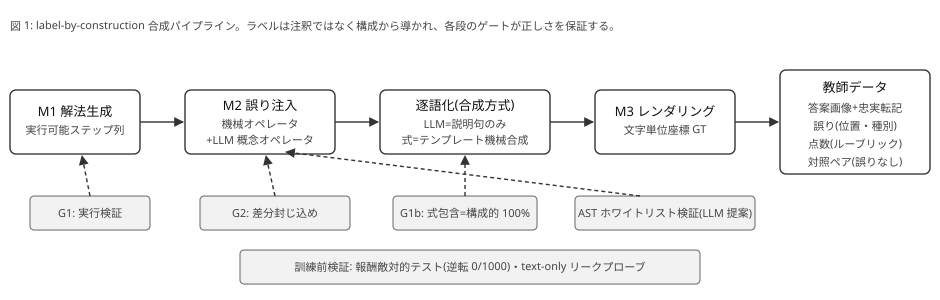
\includegraphics[width=\columnwidth]{fig/fig1_pipeline}
\caption{label-by-construction 合成パイプライン.ラベルは注釈ではなく構成から導かれる.}\label{fig:pipeline}
\end{figure}

\section{実験 1:ゼロショットから SFT へ}\label{sec:exp1}
\textbf{指標}:誤り位置 IoU@0.5 = GT 誤りごとに予測 bbox との IoU $\ge 0.5$ を正解とする比率.種別一致(マクロ)= クラス別正解率のクラス平均.幻覚誤り率 = 対照答案のうち誤りを 1 件以上報告した比率.点数完全一致 = 合計点一致率.過剰主張率 = 識別不能(ファミリ粒度 GT)の誤りのうち下位区分を断定した比率(\S\ref{sec:exp2}).

\textbf{設定}:Qwen3-VL-2B-Instruct を QLoRA(4bit・言語層のみ $r{=}16$, $\alpha{=}16$, lr $2{\times}10^{-4}$, 実効バッチ 8, 1 epoch)で 9,204 件訓練(10,000 件を pair 単位で 9,204/489/307 に分割.TITAN V 1 枚・約 2.5 時間).入力は答案画像+問題文+模範解答+採点基準,出力は JSON(忠実転記・誤りリスト・点数).評価は同一生成プールから pair 単位で隔離した held-out 200 件(事例重複なし・分布は共有)を配備形態(GGUF 8bit+llama.cpp,system プロンプトなし,temperature 0)で測定した(表~\ref{tab:sft}).

\begin{table}[t]\centering\small
\caption{ゼロショット$\rightarrow$SFT(2B,llama.cpp Q8,$n{=}200$=誤り 149/対照 51).}\label{tab:sft}
\begin{tabular}{lcc}\toprule
指標 & ゼロショット & SFT 後\\\midrule
誤り位置 IoU@0.5 & 0.000 & \textbf{0.795}\\
種別一致(9 クラス) & 0.000 & 0.647\\
検出 TPR & 1.000 & 0.980\\
検出 TNR & 0.686 & \textbf{1.000}\\
幻覚誤り率 & 0.314 & \textbf{0.000}\\
点数完全一致 & 0.345 & \textbf{0.935}\\\bottomrule
\end{tabular}
\end{table}

ゼロショット列は system プロンプト付き・絶対座標契約,SFT 列は system なし・相対座標契約であり統制は完全ではない(system 不一致だけで点数一致 0.775$\rightarrow$0.935 の差を切り分け実験で確認).ゼロショットの見かけの検出力は TPR 1.000/TNR 0.686 が示すとおり「ほぼ全答案に誤りを報告する」退化的挙動である.位置・種別は 2B/4B/8B すべてゼロショット 0 であり,SFT がこれらを立ち上げた.幻覚 0.000 は対照 51 件に対する 0 件(95\%CI 上限 $\approx$7\%)で,対照ペアの独立寄与のアブレーションは未実施である.

\section{実験 2:ラベル識別可能性}\label{sec:exp2}
\textbf{発見}:種別一致は目標 0.85 に未達で,混同は下位区分ペア内に集中し,混同方向は実行環境間で反転した.\textbf{観測同値率 $\rho$} を「あるオペレータの出力のうち他のオペレータの出力と答案表面が一致する割合」と定義し全件走査したところ,(i) 概念的誤解オペレータの $\rho=731/765=0.956$(図~\ref{fig:ident}),(ii) 誤解を語る説明句は 0/765,(iii) 積の誤解ペアは共存領域(q$\cdot$r$<$0)の 84.2\% が観測同値で,残る領域は競合オペレータが構造的に出現しない偽の識別可能領域だった.下位区分ラベルは答案の観測可能な性質ではなく\textbf{生成経路の記録}であり,これを予測ターゲットにしたことが失敗の本質である.整合性検査として,多数側タイブレークを仮定した条件付き期待値 0.7593 は実測 0.7595 とほぼ一致した(差 0.0002).この分析は LLM 概念オペレータの負の結果でもある:変異が観測に差分を落とさなければ,意味的多様性は学習可能な信号にならない.

\textbf{修正}:種別 GT を「観測から識別可能な最も細かいラベル」に写像する(観測同値な事例はファミリ,識別可能な少数事例——全誤りの 1.5\%——のみ下位区分).評価・報酬は三値:完全一致=正解/粗すぎ=部分点/\textbf{識別不能なのに下位区分=過剰主張として不正解}.写像は決定論的述語計算のみで再生成を要しない.

\begin{table}[t]\centering\small
\caption{同一計測器(held-out 200)での種別一致.}\label{tab:heldout}
\begin{tabular}{lc}\toprule
構成 & 種別一致\\\midrule
旧ラベル・旧 9 クラス評価 & 0.7595\\
\textbf{旧ラベル+推論時写像(再訓練なし)} & \textbf{0.970}\\
識別可能粒度で再訓練(3 シード) & 0.976$\pm$0.010\\\bottomrule
\end{tabular}
\end{table}

\begin{table}[t]\centering\small
\caption{未見問題群(fresh 生成 507 件,llama.cpp Q8.新モデルは parse 失敗 1 件.ファミリ間曖昧 20 件は種別指標から除外).}\label{tab:eval400}
\begin{tabular}{lcc}\toprule
指標 & 旧ラベル & 識別可能粒度\\\midrule
過剰主張率 & 0.900 & \textbf{0.010}\\
種別ファミリ 7 クラス平均 & 0.31 & 0.806\\
種別 9 クラスマクロ & 0.596 & 0.627\\
検出 TPR & \textbf{0.968} & 0.874\\
誤り位置 IoU@0.5 & \textbf{0.794} & 0.756\\
点数完全一致 & \textbf{0.909} & 0.840\\
検出 TNR/幻覚 & 1.000/0\% & 1.000/0\%\\\bottomrule
\end{tabular}
\end{table}

\textbf{再訓練は不要である}(表~\ref{tab:heldout}).推論時写像は定義上過剰主張を生じさせず(0\%),種別一致 0.970 を与える.識別可能粒度での再訓練は過剰主張を自発的に 1\% へ抑える(表~\ref{tab:eval400})が,種別一致の追加利得は確認できず,残した下位区分(訓練内被覆 1.1\%)は学習されなかった(未見 17 件に 0/17).さらに未見セットで TPR・IoU・点数が低下し(各 1 run,分散未分離),ファミリ平均 0.806 は我々の受入基準 0.90 を下回る(調査中).\textbf{実務上の推奨は旧モデル+推論時写像である}.

\section{限界}
(1) 本結果はフォントレンダリングによる手書き風合成画像内の実証であり,実筆跡への転移は今後の字形バンク収集を要する.(2) 再訓練は 3 シードで反復した(種別 0.976$\pm$0.010)が,検出・点数は天井に張り付いており分散ゼロは頑健性の証拠にならない.未見セットの比較は各 1 run である.(3) 双子ペアの変異影響ステップは独立に逐語化される.変異前ステップの字面一致は 3,000 ペアで 100\%,空白スタイル特徴の誤り判別 AUC は 0.530(偶然水準)で表層リークは検出されなかったが,網羅的検査ではない.(4) 教員間一致の実測(4 名$\times$共通 100 件)は手配段階にあり未着手で,ラベル設計の人間妥当性は未検証である.(5) 実験は中 1 数学 2 領域・単一生成器・単一モデルであり,定量的結論はこの範囲に限る.一般化できるのは検査手順である:(a) 生成経路間の観測同値率 $\rho$ を全件走査で実測し,(b) $\rho$ が高い区分を観測可能な最細粒度へ写像し,(c) 識別不能事例への断定を罰する.$\rho$ が厳密に計算可能であることは合成データ固有の利点である.

\section{おわりに}
細粒度・反実仮想ラベル付き答案データを構成により合成し,2B の小型 VLM で誤り位置・採点能力を確立した.あわせて,合成データのラベルが「構成的に正しいが観測から識別不能」でありうることを定量化し,識別可能粒度への写像と過剰主張ペナルティにより\textbf{再訓練なしで}教育的に有害な断定を除去できることを示した.コードは公開している.

\begin{thebibliography}{99}\small
\bibitem{brown1978} J.~S. Brown and R.~R. Burton. Diagnostic models for procedural bugs in basic mathematical skills. \textit{Cognitive Science}, 2(2), 1978.
\bibitem{chow1970} C.~K. Chow. On optimum recognition error and reject tradeoff. \textit{IEEE Trans. IT}, 16(1), 1970.
\bibitem{cour2011} T.~Cour et al. Learning from partial labels. \textit{JMLR}, 12, 2011.
\bibitem{deng2012} J.~Deng et al. Hedging your bets: Optimizing accuracy-specificity trade-offs in large scale visual recognition. \textit{CVPR}, 2012.
\bibitem{geifman2017} Y.~Geifman and R.~El-Yaniv. Selective classification for deep neural networks. \textit{NeurIPS}, 2017.
\bibitem{gupta2016} A.~Gupta et al. Synthetic data for text localisation in natural images. \textit{CVPR}, 2016.
\bibitem{kim2022} G.~Kim et al. OCR-free document understanding transformer. \textit{ECCV}, 2022.
\bibitem{zheng2025} C.~Zheng et al. ProcessBench: Identifying process errors in mathematical reasoning. \textit{ACL}, 2025.
\bibitem{daheim2024} N.~Daheim et al. Stepwise verification and remediation of student reasoning errors with large language model tutors. \textit{EMNLP}, 2024.
\bibitem{nath2025} O.~Nath et al. Can vision-language models evaluate handwritten math? \textit{ACL}, 2025.
\bibitem{khrulev2025} R.~Khrulev. CHECK-MAT. arXiv:2507.22958, 2025.
\bibitem{maeda2026} K.~Maeda and N.~Okazaki. JaWildText. arXiv:2603.27942, 2026.
\bibitem{mizumoto2023} A.~Mizumoto and M.~Eguchi. Exploring the potential of using an AI language model for automated essay scoring. \textit{RMAL}, 2(2), 2023.
\bibitem{liu2024} R.~Liu et al. Best practices and lessons learned on synthetic data. \textit{COLM}, 2024.
\end{thebibliography}

\appendix
\section{生成例}
図~\ref{fig:example} に実生成例(問題「$4x-5=-10$」,概念/移項を s2 に注入,点数 GT 3/10)を示す.注入は「$+5$」$\rightarrow$「$-5$」の 1 文字で,機械オペレータも同一表面を生む=観測同値の実例である.

\begin{figure}[t]\centering
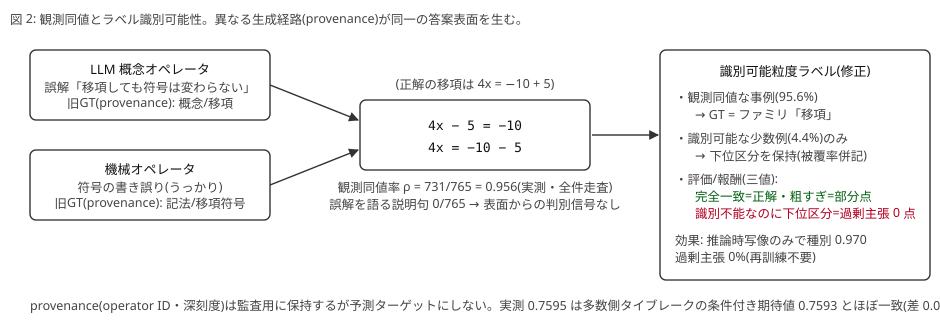
\includegraphics[width=\columnwidth]{fig/fig2_identifiability}
\caption{観測同値とラベル識別可能性(走る例で統一).}\label{fig:ident}
\end{figure}
\begin{figure}[t]\centering
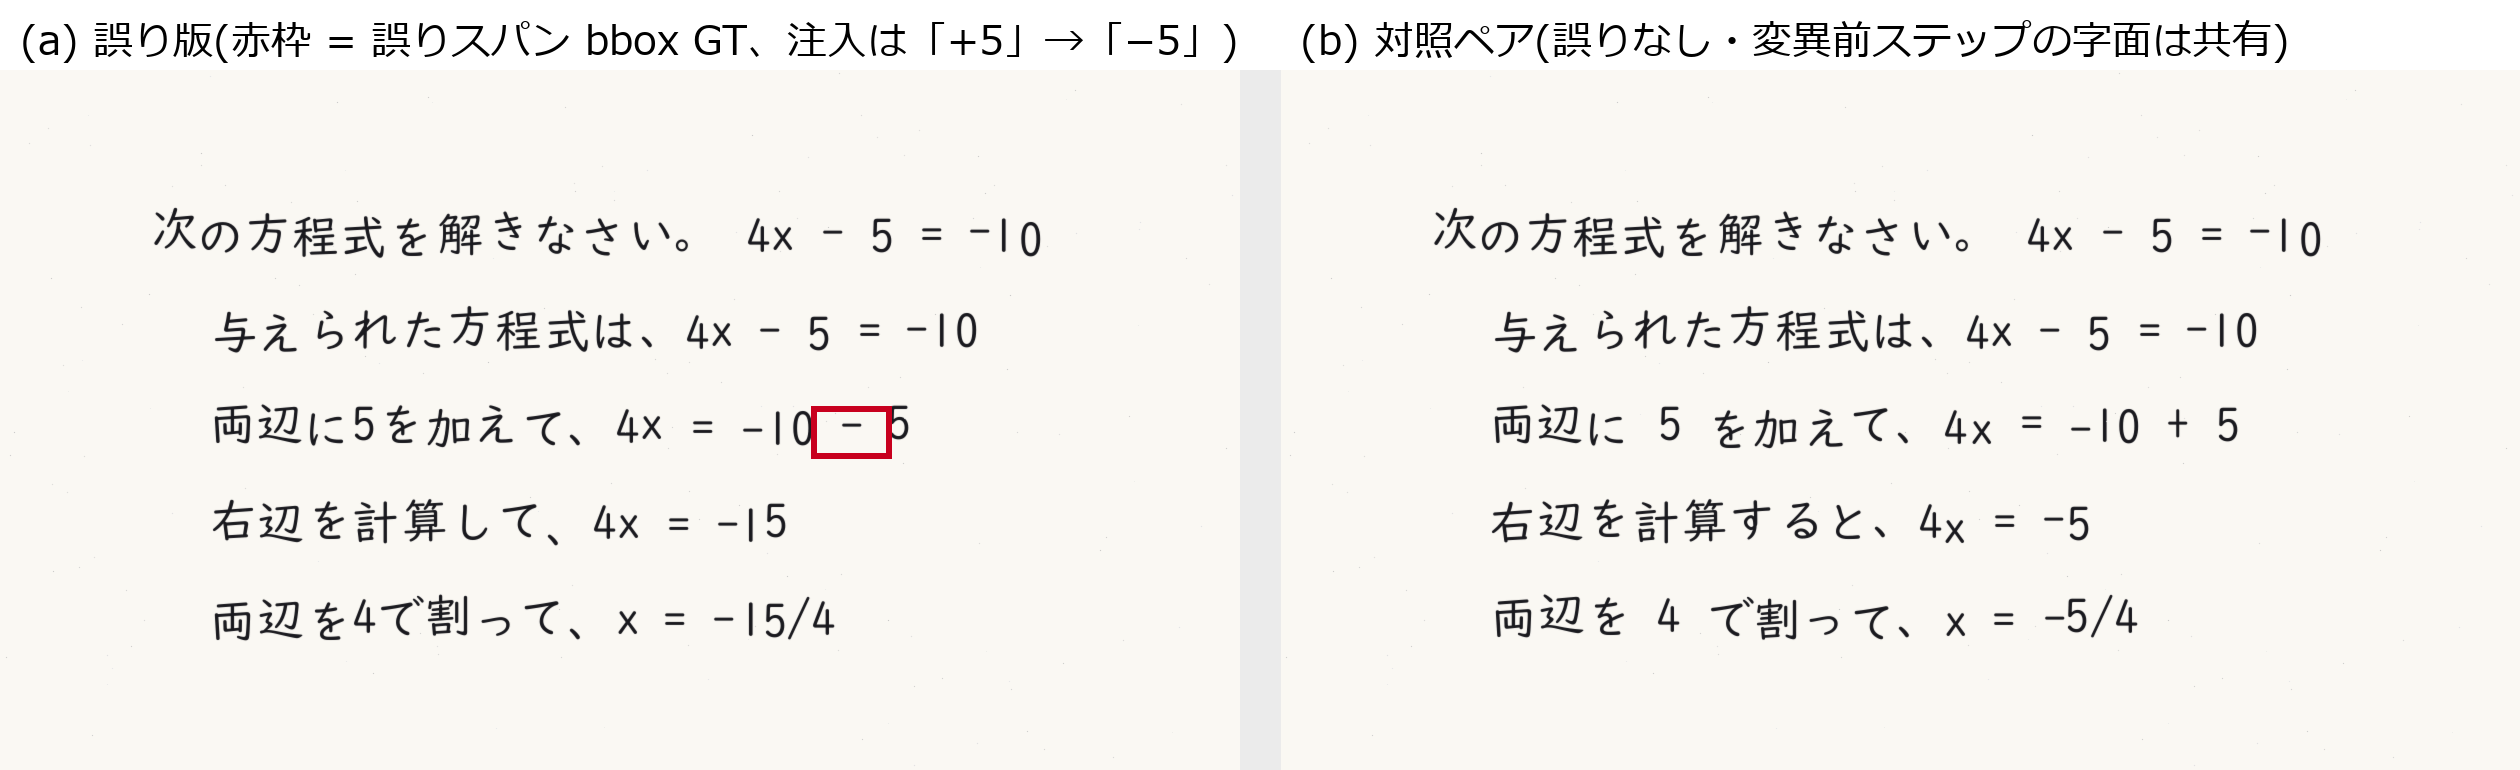
\includegraphics[width=\columnwidth]{fig/fig3_example_pair}
\caption{実生成例.(a) 誤り版(赤枠=bbox GT),(b) 対照ペア.}\label{fig:example}
\end{figure}

\end{document}
